\section{Desarrollo}

\subsection{Planteo del Sistema}


La temperatura en un punto $t_{(j,k)}$, con $j \in [0, m]$ y $k \in [0, n)$ estará determinado por la ecuación de Laplace descripta a continuación:


$$ \frac{\partial^{2}T(r,\theta)}{\partial r^{2}} + \frac{1}{r} \frac{\partial T(r,\theta)}{\partial r} + \frac{1}{r^{2}} \frac{\partial^{2}T(r,\theta)}{\partial \theta^{2}} = 0$$\\

Sin embargo utilizaremos una aproximación de esta función que depende de los cuatro puntos que rodean a $t_{(j,k)}$:


$$ \frac{t_{(j-1,k)} - 2t_{(j,k)} + t_{(j+1,k)}}{\Delta_{r} ^{2}} + \frac{1}{r} \frac{t_{(j,k)} - t_{(j-1,k)}}{\Delta_{r}} + \frac{1}{r^{2}} \frac{t_{(j,k-1)} - 2t_{(j,k)} + t_{(j,k+1)}}{\Delta_{\theta} ^{2}} = 0$$

Despejamos las incógnitas $t_{(j,k)}$, $t_{(j+1,k)}$, $t_{(j-1,k)}$, $t_{(j,k+1)}$ y $t_{(j,k-1)}$ para obtener una ecuación (un sistema de ecuaciones) que dependa de ellas. Resulta la siguiente fórmula:



$$  t_{(j,k)} (-\frac{2}{\Delta^2_r}+\frac{1}{r \Delta_r}-\frac{2}{r^2 \Delta^2_\theta}) + t_{(j+1,k)} (\frac{1}{\Delta^2_r}) + t_{(j-1,k)} (\frac{1}{\Delta^2_r}-\frac{1}{r \Delta_r}) + t_{(j,k+1)} (\frac{1}{r^2 \Delta^2_\theta}) + t_{(j,k-1)} (\frac{1}{r^2 \Delta^2_\theta}) = 0$$ \\


Una vez planteadas estas ecuaciones para cada $ t_{(j,k)} $, resolvemos que el sistema $Ax = b$ estará formado por $n*m$ ecuaciones con la misma cantidad de incógnitas. El valor lo justificamos debido a la cantidad de combinaciones entre los índices j y k (cantidad de ángulos por cantidad de radios). Otra forma de razonar este resultado es pensando que en cada anillo generado por la partición del horno en \textbf{\textit{m + 1}} radios, habrá \textbf{\textit{n}} incógnitas generadas a su vez por la particion en ángulos. \\
Esta cantidad incluye los valores $t_{(0,k)}$ y $t_{(n-1,k)}$ (los valores de temperatura en la pared interior y exterior respectivamente), por lo que en sus ecuaciones habrá un único coeficiente con valor 1 en la posición que corresponde a estas incógnitas y su valor b será el que se pase por parámetro. Para el resto de los $t_{(j,k)}$ los coeficientes corresponderan a los coeficientes descriptos en la ecuación de arriba, y su b será cero, también respetando dicha ecuación.


%-------------------------------------------------------------------------

\subsection{Orden de los coeficientes}

%que es una matriz banda

Para conseguir una matriz banda, decidimos ordenar los coeficientes de manera creciente respecto al índice de los radios \textbf{\textit{j}} y luego respecto a \textbf{\textit{k}} el índice de los ángulos. Para ilustrar el orden impuesto, exponemos el siguiente ejemplo:

Sea $\Delta_{r} = 1$,  $\Delta{\theta} = \frac{\pi}{2}$, $\textbf{\textit{m + 1}} = \textbf{\textit{n}} = 4$ el orden resultante será 

$$ t_{(0,0)} t_{(0,1)} t_{(0,2)} ...... t_{(2,0)} t_{(2,1)} t_{(2,2)} $$


A continuación explicamos por qué este orden para las filas y columnas de la matriz genera una matriz banda.

En cada fila, salvo las primeras n y las últimas n, el coeficiente que acompaña a la incognita $T_{(j,k)}$ de la ecuación va a ser el elemento de la diagonal. Además, en cada fila van a aparecer los coeficientes no nulos $a_{(j-1,k)}$,$a_{(j+1,k)}$,$a_{(j,k-1)}$ y $a_{(j,k+1)}$.
Los coeficientes $a_{(j-1,k)}$ y $a_{(j+1,k)}$ van a estar a una distancia de m+1 elementos de la diagonal, y los coeficientes $a_{(j,k-1)}$ y $a_{(j,k+1)}$ van a estar siempre a una distancia menor. Como esto se cumple para todas las filas, siempre van a haber dos diagonales formadas por los coeficientes mas lejanos al coeficiente de la diagonal, como se ve en la siguiente figura:

\begin{figure}[h]
  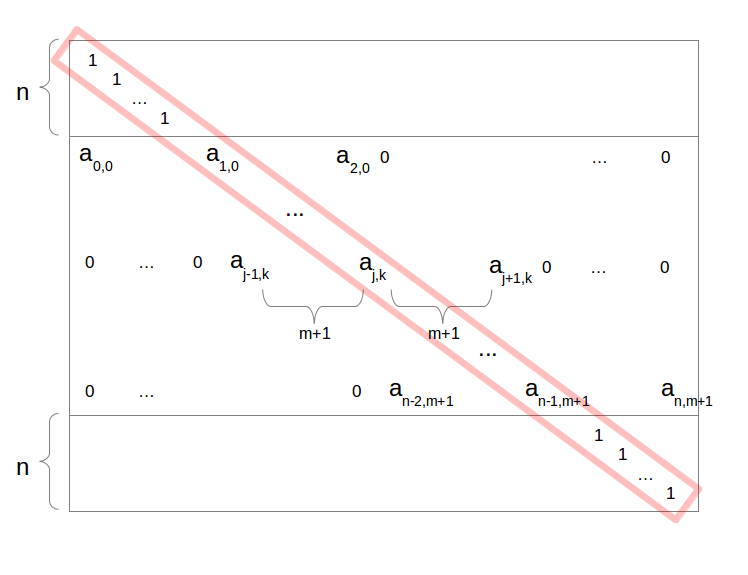
\includegraphics[scale=0.4]{imagenes/figura1.png}
  \caption{La figura}
  \label{fig:corteHorno}
\end{figure}

%---------------------------------------------------------------------
\newpage
\subsection{Análisis de Coeficientes}
A partir de las aproximaciones de las derivadas parciales de la función $T$ distribuimos los términos para conocer los coeficientes asociados a cada punto del cual depende el valor de la temperatura que queremos conocer para un $j,k$ dado. Se debe cumplir la siguiente ecuación: \\
$$t_{(j-1, k)} (\frac{1}{\Delta^2_r}-\frac{1}{r \Delta_r}) +
t_{(j, k)} (-\frac{2}{\Delta^2_r}+\frac{1}{r \Delta_r}-\frac{2}{r^2 \Delta^2_\theta}) + 
t_{(j+1, k)} (\frac{1}{\Delta^2_r}) + 
t_{(j, k-1)} (\frac{1}{r^2 \Delta^2_\theta}) +
t_{(j, k+1)} (\frac{1}{r^2 \Delta^2_\theta}) = 0 $$ \\

Analizamos los casos en que los coeficientes obtenidos a partir de la discretización de las derivadas parciales asociados a cada punto se anulan, es decir, para que $r, \Delta_r,$ y $\Delta_\theta$ el coeficiente se anula. \\
Para el coeficiente asociado a $t_{(j-1, k)}$, $r$ debe valer $\Delta_r$. Como $r_j = (j \Delta_r) + r_i$ esto se cumple si $j$ vale 1 y $r_i$ vale cero, o $j$ vale cero y $r_i$ vale $\Delta_r$. Para el primer caso, significa que el horno no tiene radio interno, mientras que la segunda no puede suceder puesto que la ecuación la cumplen solo las temperaturas entre el radio interno y el externo (no incluidos) y si $j$ vale cero, indica que es el radio interno.
Para los coeficientes de $t_{(j+1, k)}$, $t_{(j, k-1)}$ y $t_{(j, k+1)}$, los coeficientes nunca se anulan. \\
Por último, para el coeficiente asociado a $t_{(j, k)}$, desarrollamos las sumas e igualamos a cero. \\
$$\frac{-2r^2 \Delta^2_\theta + r \Delta_r \Delta^2_\theta - 2 \Delta^2_r}{\Delta^2_r r^2 \Delta^2_\theta} = 0$$\\
El término inferior nunca se anula, por lo que debería anularse el término superior. Observamos que corresponde a una función cuadrática siendo $r$ la variable. Desarrollamos la fórmula de Bhaskara obteniendo: \\
$$r = \frac{\Delta_r}{4} \pm \frac{\sqrt{\Delta^2_r \Delta^4_\theta - 16 \Delta_\theta \Delta^2_r}}{4 \Delta^2_\theta}$$ \\
El análisis se vuelve muy complicado, pero nos valemos de saber que para que el planteo tenga sentido, $r$ debe ser mayor o igual que $\Delta_r$.
El segundo miembro es siempre positivo, por lo que si se le resta algo positivo a $\frac{\Delta_r}{4}$, seria aún menor, por lo tanto solo queda analizar el caso en que se suman los términos. Para que se cumpla la condición $\Delta_r \leq r$, queremos encontrar los $\Delta_r$ y $\Delta_\theta$ tal que: \\
$$\frac{3 \Delta_r}{4}  \leq \frac{\sqrt{\Delta^2_r \Delta^4_\theta - 16 \Delta_\theta \Delta^2_r}}{d \Delta^2_\theta} $$ \\
Para este fin, utilizamos la página web $www.wolframalpha.com$ para encontrar las soluciones al problema, las cuales indican que si $\Delta_r$ es positivo, $\Delta_\theta$ debe ser menor a cero y viceversa. Por lo tanto, el coeficiente se anula solamente para valores que no tienen sentido dentro del problema. \\
%http://www.wolframalpha.com/input/?i=sqrt%28x^2+y^4+-+16+x^2+y%29+%2F+%284*y^2%29+%3E%3D+3x%2F4
Con este análisis, concluimos que los coeficientes obtenidos de la ecuación no se anulan en los casos en que el problema planteado tiene sentido.

%---------------------------------------------------------------------

\subsection{Análisis de Pivoteo}

Para justificar que en la matriz banda no se produce pivoteo al aplicarse el algoritmo de Eliminación Gaussiana, procedemos a demostrar que la matriz banda es diagonal dominante. Con esto llegamos a la conclusión de que es no singular. Con esto se tiene  que la matriz tiene factorización LU, con lo cual no se produce pivoteo en la E.G.


%---------------------------------------------------------------------


\subsubsection{A es diagonal dominante}
Queremos ver que A es diagonal dominante, es decir, que se cumple la siguiente inecuación:\\
$$\mid \frac{1}{\Delta^2_r}-\frac{1}{r \Delta_r}\mid +
\mid \frac{1}{\Delta^2_r} \mid + 
\mid \frac{1}{r^2 \Delta^2_\theta} \mid +
\mid \frac{1}{r^2 \Delta^2_\theta} \mid
\leq \mid -\frac{2}{\Delta^2_r}+\frac{1}{r \Delta_r}-\frac{2}{r^2 \Delta^2_\theta} \mid$$  \\
Primero, nos deshacemos de los módulos. El primer término es negativo solo cuando $r < {\Delta_r}$, pero esto no sucede debido a que $r= j \Delta_r + r_i$, con $j$ natural y $r_i$ real positivo. El resto de los términos a la izquierda de la desigualdad tambien son positivos debido a que todas las viariables estan elevadas al cuadrado, por lo tanto es equivalente no tomar módulo para estos términos. \\
Para el término de la derecha, $-\frac{2}{r^2 \Delta^2_\theta}$ siempre es negativo, por lo que para que el término sea positivo, $-\frac{2}{\Delta^2_r}+\frac{1}{r \Delta_r}$ debe de ser necesariamente positivo. Sin embargo, esto solo puede ocurrir cuando $r < \frac{\Delta_r}{2}$, por lo que siempre resulta negativo por el argumento anterior. De este modo, si multiplicamos este término por -1, obtenemos un número positivo. La inecuación resultante es: \\ 
$$ \frac{1}{\Delta^2_r}-\frac{1}{r \Delta_r} +  
\frac{1}{\Delta^2_r} + 
\frac{1}{r^2 \Delta^2_\theta} +
\frac{1}{r^2 \Delta^2_\theta}
\leq \frac{2}{\Delta^2_r}-\frac{1}{r \Delta_r}+\frac{2}{r^2 \Delta^2_\theta}$$ \\

Sumamos los términos y obtenemos: \\
$$\frac{2}{\Delta^2_r}-\frac{1}{r \Delta_r}+\frac{2}{r^2 \Delta^2_\theta} \leq \frac{2}{\Delta^2_r}-\frac{1}{r \Delta_r}+\frac{2}{r^2 \Delta^2_\theta}$$ \\
Podemos observar que se cumple la inecuación como queríamos demostrar, y en particular, vale la igualdad.


%---------------------------------------------------------------------

\subsubsection{A es no singular}
Dada la matriz A diagonal dominante, veamos que A es no singular.
Por absurdo supongamos que es singular, esto es, $\exists x\neq 0$ tal que $x \in Nu(A)$.
Como el vector es distinto a cero, existe una coordenada que es mayor al resto. Llamémosla $x_{k}$.


Del sistema de ecuaciones Ax, tomemos la ecuación k, que tiene esta forma:                  

$$ a_{(k, 1)} * x_{1} + a_{(k, 2)} * x_{2} +... + a_{(k, n)} * x_{n} = 0 $$\\

Luego despejamos el término k y aplicamos módulo:\\

 $$ \mid a_{(k, k)} * x_{k} \mid  =  \left \arrowvert - \sum_{j=1,j\neq k}^{n}  a_{(k,j)} * x_{j} \right \arrowvert $$

 $$ \mid a_{(k, k)}\mid * \mid x_{k} \mid \leq \sum_{j=1,j\neq k}^{n} \mid a_{(k,j)}\mid * \mid x_{j} \mid $$


 $$ \mid a_{(k, k)}\mid  = \sum_{j=1,j\neq k}^{n} \mid a_{(k,j)}\mid *  \frac{\mid x_{j} \mid}{\mid x_{k} \mid}$$\\

Anteriormente probamos que A es diagonal dominante y que en particular vale la igualdad. Como cada elemento de la sumatoria (que vale exactamente $a_{(k, k)}$) es multiplicado por $\frac{\mid x_{j} \mid}{\mid x_{k} \mid}$ $\leq 1$, disminuyen su valor, con lo que la sumatoria se reduce y resulta:\\

$$\mid a_{(k,k)} \mid < \sum_{j=1, j\neq k}^{n}\mid a_{(k,j)} \mid $$\\

Lo que es absurdo, pues A era diagonal dominante. El absurdo provino de suponer que A es singular. Luego vale que A es no singular.

%---------------------------------------------------------------------

\subsubsection{A tiene factorización LU}


Como sabemos que A es diagonal dominante, todas sus submatrices tambien lo cumplen. Por lo que probamos antes, todas sus submatrices son no singulares. 

Por la propiedad: A tiene sus submatrices principales no singulares $\Leftrightarrow$ tiene factorización LU.

Entonces nuestra matriz tiene factorización LU, y la eliminación gaussiana se puede hacer sin pivoteo.


%---------------------------------------------------------------------


\subsection{Implementación de los algoritmos}

Nuestro programa comienza obteniendo los parámetros que son: un archivo de entrada, uno de salida y el método de triangulación. 

Del archivo de entrada obtenemos los radios interno y externo, el m y n, la isoterma buscada, la cantidad de instancias y luego las temperaturas conocidas para cada instancia.  

Luego calculamos los valores de los coeficientes de cada ecuación y creamos una matriz A $\in$ $R^{n*(m+1) X n*(m+1)}$ cuyos elementos estan ordenados con el orden que mencionamos anteriormente, para que sea una matriz banda.

Dependiendo del método que corresponde, se hace la eliminación gaussiana o la factorización LU.

\subsubsection{Implementación de Eliminación Gaussiana}

Con la matriz A ya cargada (esto se hace una única vez), para cada instancia del problema, se carga un vector de términos independientes b $\in$ $R^{n*(m+1) X 1}$. La matriz A nunca se modifica (se hacen copias) para que se pueda usar la misma en cada instancia. 

Para cada fila_{i}, se recorren los elementos de las filas inferiores (fila_{j} con i>j) restandoles la fila_{i} multiplicada por un coeficiente conveniente para que los elementos de fila_{j} queden en 0 hasta la columna iésima. Para los elementos que ya se sabe que deben valer 0 no se hace la cuenta, para evitar que aparezcan valores muy chicos y haya errores de precisión.

Una vez que conseguimos la matriz triangulada, llamamos a la función de Backward Substitution que toma una matriz triangular superior y el vector b. Éste recorre las filas en orden ascendente despejando las incógnitas. 

Vamos guardando los valores del vector X hallados de cada sistema de ecuaciones AX = b, en el archivo de salida. La complejidad de este algoritmo resulta ser O($(n*(m+1))^{3}$) por cada sistema. 

%justificar por que es esa la comlejidad.

\begin{algorithm}
\caption{Eliminación Gaussiana}\label{euclid}
\begin{algorithmic}[1]

  \Function{GaussianElimination}{A, b}\Comment{con $A \in R^{(nxm)*(nxm)}$, $b \in R^{nxm}$}

    \State $\textit{U} = \text{A.clone()}$

    \For {$actual\_row = 0$ to $U.rows() - 2$}
      \If {$U(actual\_row, actual\_row) == 0$} 
        \Return
      \EndIf

      \For {$row = actual\_row + 1$ to $U.rows() - 1$}
          \State $coefficient = U(row, actual\_row) / U(actual\_row, actual\_row)$
          \For {$col = actual\_row$ to $U.cols() - 1$}
            \If {$col == actual\_row$}  
              \State $U(row,col) = 0$
            \Else
              \State $U(row, col) = U(row, col) - coefficient * U(actual\_row, col)$
            \EndIf
          \EndFor

          \State $b(row) = b(row) - (coefficient * b(actual\_row)$
      \EndFor    
    \EndFor

  \EndFunction

\end{algorithmic}
\end{algorithm}

\begin{algorithm}
\caption{Backward Substitution}\label{euclid}
\begin{algorithmic}[1]

  \Function{Backward Substitution}{U, b}\Comment{con $U \in R^{(nxm)*(nxm)}$, $b \in R^{nxm}$}

    \State $\textit{X} = \text{Mat(U.rows())}$

    \For {$i = U.rows() - 1$ to $0$}
      \State $acum = 0.0$

      \For {$j = i+1$ to $U.rows() - 1$} 
        \State $acum = acum + U(i, j) * X(j)$
      \EndFor

      \State $X(i) = b(i) - acum / U(i, i)$

    \EndFor
      
  \EndFunction

\end{algorithmic}
\end{algorithm}


\subsubsection{Implementación de Factorización LU}

Por única vez y en un principio, con la matriz A ya cargada, se obtiene la matriz LU que es del mismo tamaño:
De la misma manera que en la eliminación gaussiana, se obtiene la matriz triangulada U ,y tambien la matriz de coeficientes L. 

\begin{algorithm}
\caption{Generación de Matriz LU}\label{euclid}
\begin{algorithmic}[1]

  \Function{GetLU}{A, LU}\Comment{con $A \in R^{(nxm)*(nxm)}$, $LU \in R^{(nxm)*(nxm)}$}

    \State $\textit{LU} = \text{A.clone()}$

    \For {$actual\_row = 0$ to $LU.rows() - 2$}
      \If {$LU(actual\_row, actual\_row) == 0$} 
        \Return
      \EndIf

      \For {$row = actual\_row + 1$ to $LU.rows() - 1$}
          \State $coefficient = LU(row, actual\_row) / LU(actual\_row, actual\_row)$
          \For {$col = actual\_row$ to $LU.cols() - 1$}
            \If {$col == actual\_row$}  
              \State $LU(row,col) = coefficient$
            \Else
              \State $LU(row, col) = LU(row, col) - coefficient * LU(actual\_row, col)$
            \EndIf
          \EndFor

      \EndFor    
    \EndFor

  \EndFunction

\end{algorithmic}
\end{algorithm}


Sabemos que los elementos de la diagonal de L son todos 1 y es triangular inferior y la U es triangular superior. Entonces en la parte triangular superior de la matriz LU se guarda la U, y en la inferior (salvo la diagonal) se guarda la L.

Para cada instancia, resolvemos el sistema de ecuaciones AX = b haciendo dos backward substitution. 

El primero resuelve el sistema Ly = b despejando las incógnitas en forma descendiente de una matriz que es triangular inferior. Utiliza de la matriz LU solamente los elementos que corresponden a la L, teniendo en cuenta que los elementos de la diagonal deberían ser 1.


\begin{algorithm}
\caption{Backward Substitution LU}\label{euclid}
\begin{algorithmic}[1]

  \Function{Backward Substitution LU}{LU, b}\Comment{con $LU \in R^{(nxm)*(nxm)}$, $b \in R^{nxm}$}

    \State $\textit{X} = \text{Mat(LU.rows())}$
    \State $X(0) = b(0)$

    \For {$i = 1$ to $LU.rows() - 1$}
      \State $X(i) = b(i)$

      \For {$j = 0$ to $i - 1$} 
        \State $X(i) = X(i) - LU(i,j)*X(j)$
      \EndFor

    \EndFor
      
  \EndFunction

\end{algorithmic}
\end{algorithm}

El segundo usa el mismo algoritmo que el backward substitution de la eliminación gaussiana para resolver el sistema Ux = y y hallar las incógnitas del sistema original. 

Vamos guardando los valores del vector X hallados de cada sistema de ecuaciones AX = b, en el archivo de salida. La complejidad de este algoritmo resulta ser O($(n*(m+1))^{3}$) para la obtención de la matriz LU (la primera instancia) y O($(n*(m+1))^{2}$)
por instancia posterior.
%por que esta complejidad?


\subsubsection{Obtención de la isoterma}

El algoritmo que usamos para obtener los valores de los radios de la isoterma buscada, que usa la solución del sistema ya resuelto por medio de eliminación gaussiana o factorización LU, es el siguiente:

\begin{algorithm}
\caption{Obtención del radio de la isoterma}\label{euclid}
\begin{algorithmic}[1]

  \Function{getIsotermRadiusValues}{X, angles, isoterm, delta_r, ri}

  \Comment{con $X\_s \in R^{nxm}$, $angles \in N$, $isoterm, delta\_r, ri \in R$}
    \State $X = X\_s.reverseOrder()$
    \State $isotermRadious[angles]$

    \For {$i = 0$ to $angles - 1$}
      \State $isotermRadius[i] = -1$
    \EndFor

    \For {$j = 0$ to $X.rows() - angles - 1$}
      \If {$X(j) >= isoterm \wedge X(j+angles) <= isoterm$}
       \State $isotermRadius[j \% angles] = (ri + (j / angles)*delta\_r + (((X(j) - isoterm) * delta_r)/ (X(j) - X(j+angles)) ))$
      \EndIf
    \EndFor

  \EndFunction

\end{algorithmic}
\end{algorithm}

%explicar mas o menos este algoritmo y que complejidad tiene
Primero invertimos el orden del vector solución para que empiece a tomar los valores más internos y luego los mas externos. Asignamos valores centinelas al vector $isotermRadius$, donde guardaremos el valor del radio de la isoterma para cada angulo. Si no se encuentra la isoterma para un angulo dado, el vector tendrá un -1 para ese angulo, indicando un error. Esto puede suceder cuando el valor externo de la temperatura es estrictamente mayor al valor de la isoterma buscada. \\
\begin{wrapfigure}{l}{0.5\textwidth}
  \vspace{-20pt}
  \begin{center}
    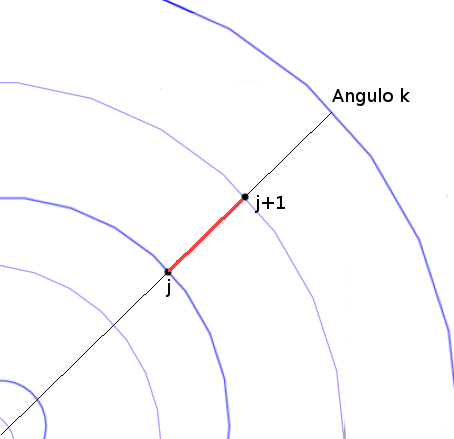
\includegraphics[scale= 0.6]{imagenes/radiosLimpio.png}
  \end{center}
  \vspace{-20pt}
  \caption{Seccion de horno}
  \vspace{-10pt}
  \label{fig:Exp3}
\end{wrapfigure}

Luego se itera para cada angulo del horno, el valor de la temperatura para el punto $j$ y el $j+1$ como se ve en el gráfico, buscando si entre esos dos valores se encuentra la isoterma buscada. Una vez encontrados esos puntos, se le asigna el valor del radio estimado de la isoterma. Para esto, utilizamos una regla de tres simple: $ri + j *\Delta_r $ es el valor del radio para el punto $j$. Luego planteamos que, si entre el punto $j$ y el $j+1$ (que tienen una diferencia de radio $\Delta_r$) hay una diferencia de temperatura de $T(j) - T(j+1)$, cual sería el valor del radio si la diferencia es de $T(j) - isoterma$. Luego se le suma ese valor al radio del punto $j$.\\
Para el caso de la implementación, el punto siguiente ($j+1$) se calcula como $j+angulos$ porque en la matriz columna $X$, se guardan las temperaturas de los primeros $n$ radios más internos, luego los $n$ radios que le siguen, así sucesivamente hasta llegar a los $n$ radios externos. Por esta misma razón, se toma $j \% angles$ como subindice para el vector.\\
Para el experimento en que la instancia tiene los valores de la temperatura interna menores a los de la externa, la condición de la línea 5 deben darse vuelta las desigualdades (puesto que estamos utilizando fuertemente que las temperaturas internas son mayores a las externas).\\

Para una instancia dada, se tienen $n$ angulos y $m+1$ radios. La función de la línea 3 (reverseOrder()) devuelve una copia del vector solución pero con los valores ordenados al revéz. Esto tiene un costo de O($n*(m+1)$). El $for$ de la linea 4 tiene complejidad O($n$) y el $for$ de la linea 6 tiene complejidad O($n*(m+1)$), puesto que se recorren todos los radios de todos los angulos. Las operaciones de ambos $for$ don O($1$). Como resultado final, la complejidad del algoritmo es O($n*(m+1)$). Se puede disminuir la complejidad a O($n*log(m+1)$) si se hiciera una busqueda binaria para encontrar los radios entre los que se encuentra la isoterma. Optamos por no tomar esta opción por simplicidad ya que el recorrido de los indices no es trivial, además que la mejora temporal introducida por el logaritmo no mejora la complejidad total dado que los algoritmos de eliminación Gaussiana y LU son del orden cúbico.




%---------------------------------------------------------------------

\subsection{Problemas que nos encontramos durante el desarrollo}

\begin{itemize}
\item Nos encontramos con problemas a la hora de cargar la matriz A de coeficientes. Lo solucionamos realizando ejemplos de un tamaño razonable en papel, y chequeando a mano que las distintas filas estuvieran bien cargadas.

\item Problemas de precisión numérica. Inicialmente los resultados de los\ tests diferían con los resultados de la cátedra. Debido a los problemas inherentes a la aritmética de punto flotante, comenzamos experimentando con distintas maneras de realizar la sumatoria (ordenando los números de mayor a menor y de menor a mayor), ya que pensabamos que estabamos arrastrando un error. Descubrimos que las distintas maneras de realizar las sumatorias diferían en menos de $0,00001$, por lo que concluímos que no estabamos arrastrando errores en las cuentas. Finalmente descubrimos que el error estaba en que la variable $m$ en realidad era $m+1$, y no teníamos eso en cuenta a la hora de calcular $\Delta r$.

\end{itemize}